\documentclass[10pt,conference,compsocconf]{IEEEtran}

\usepackage{hyperref}
\usepackage{graphicx}
\usepackage{amsmath}
\usepackage{booktabs}
\usepackage{xcolor}

% Figures are drawn by the scripts of experiments/ into report/figures/.
\graphicspath{{figures/}}
\newcommand{\Pmiss}{P_{\mathrm{miss}}}
\newcommand{\Pfa}{P_{\mathrm{fa}}}
\newcommand{\todo}[1]{\textcolor{red}{[TODO: #1]}}

\begin{document}
\title{Beyond \texorpdfstring{$3\times3$}{3x3}: auditing the binary pattern channel for copy detection patterns across prints, sessions and attacks}

\author{
  Elie Bussod, Gabin Prunet, Antoine Mandly\\
  \textit{CS-433 Machine Learning, EPFL, Switzerland}
}

\maketitle

\begin{abstract}
  \todo{write last: problem, what we measure, main numbers before / after, what it means for provable guarantees.}
\end{abstract}

% ---------------------------------------------------------------------------- 0.5 page
\section{Introduction}
\todo{copy detection patterns and estimation attacks; the binary pattern channel (BPC) model of Tutt~\cite{tutt2025thesis} and its headline result.}

\todo{the precise problem: three assumptions of the model never tested on real data; threshold and $\mu$ chosen on the test set; no confidence intervals; one dataset and one kind of attack.}

\todo{our three contributions and the two datasets~\cite{chaban2022variability,khermaza2021scantrust}. We answer the open questions of the thesis (chap.~7).}

% ---------------------------------------------------------------------------- 0.9 page
\section{Model and methods}
\label{sec:methods}
\todo{BPC: codebook $P_b(\omega)$, assumptions, PLL and mask~\cite{tutt2024tifs,tutt2024provable}.}

\todo{what the $3\times3$ model misses: reproducible part $\rho$, image effect; flip models with a larger context (5$\times$5 table with back-off, comparison models). The idea of a printer model with context comes from halftoning~\cite{pappas1995printer}.}

\todo{thresholds: conformal threshold on originals~\cite{bates2023conformal}, recalibration.}

\todo{a fake is a second pass through the channel (4-line box)~\cite{phanho2014graphical,baras2012eusipco}.}

% ---------------------------------------------------------------------------- 0.6 page
\section{Data and protocol}
\label{sec:data}
\todo{Indigo (mobile, scanner, variability) and Scantrust; what each dataset allows (4-line table).}

\todo{binarization; blocks grouped by template; development subsets; methods frozen before any test fake was read.}

\todo{operating points and intervals: Clopper-Pearson (one image per template), bootstrap on templates for repeated prints~\cite{kish1965survey,cameron2008bootstrap}.}

% ---------------------------------------------------------------------------- 1.5 pages
\section{Results}
\label{sec:results}

\begin{figure*}[t]
  \centering
  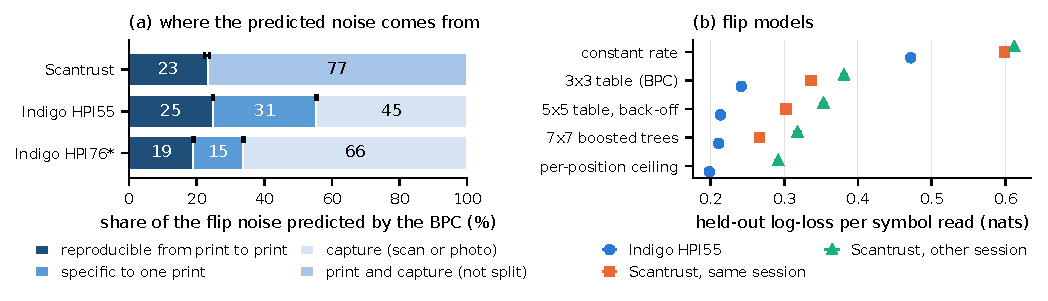
\includegraphics[width=\textwidth]{fig1.pdf}
  \caption{What the $3\times3$ BPC model misses, on originals only.
    (a)~Share of the flip noise predicted by the BPC that is reproducible from one print
    of a template to the next (template), reproducible between reads of one print only
    (print), or new at each capture (capture). Error bars: 95\,\% bootstrap intervals on
    templates for $\rho$ between prints and between reads. *HPI76: prints of session~1,
    scans of session~0. Scantrust has no repeated scan, so print and capture are not split.
    (b)~Log-loss per symbol read (nats, lower is better) of flip models on templates never
    used for fitting, with 95\,\% bootstrap intervals on templates (most are smaller than
    the markers). The per-position ceiling uses the other reads of the same template: it is
    a bound, not a usable model.}
  \label{fig:noise}
\end{figure*}

\subsection{What the \texorpdfstring{$3\times3$}{3x3} model misses}
Under the BPC, which symbols of a template flip is pure chance once their $3\times3$
patterns are known: two prints of the same template should not flip the same symbols
more often than the codebook predicts. They do. Between two prints, a share
$\rho = 0.248$ (95\,\% CI 0.247--0.250) of the flip noise predicted by the BPC is
reproducible on the Indigo HPI55 printer, 0.190 on HPI76 and 0.232 on Scantrust
(Fig.~\ref{fig:noise}a), against $|\rho| < 0.0003$ for 200 draws from the BPC on the same
templates. With four scans of each print, the noise of HPI55 splits into 25\,\% that comes
with the template, 31\,\% specific to one print and 45\,\% from the scan. The reproducible
part is almost zero on reliable patterns and largest for patterns with a flip
probability between 0.3 and 0.7. The flip rate also varies from one image to the next
8 to 15 times more than the binomial noise on Indigo scans, but only about as much as the
binomial noise on Scantrust (ratio 0.90, CI 0.75--1.05).

A larger context recovers most of the reproducible part (Fig.~\ref{fig:noise}b). A
$5\times5$ table that backs off to the $3\times3$ codebook when a context is rare, fitted on
originals of other templates, cuts the held-out log-loss of the $3\times3$ table by 11.7\,\%
on Indigo, 10.1\,\% on Scantrust in the same session and 7.3\,\% in another session, and
roughly halves the reproducible part left over ($\rho$ from 0.246 to 0.138 on Indigo, from
0.169 to 0.075 on Scantrust). Boosted trees on a $7\times7$ window add little on Indigo but
more on Scantrust (20.8\,\% and 16.6\,\%). The gain carries over to other print sessions of
the same printer (13.2\,\% and 11.4\,\%) but not to the other printer (2.7\,\%).

\subsection{A threshold holds for one print run only}
\begin{figure*}[t]
  \centering
  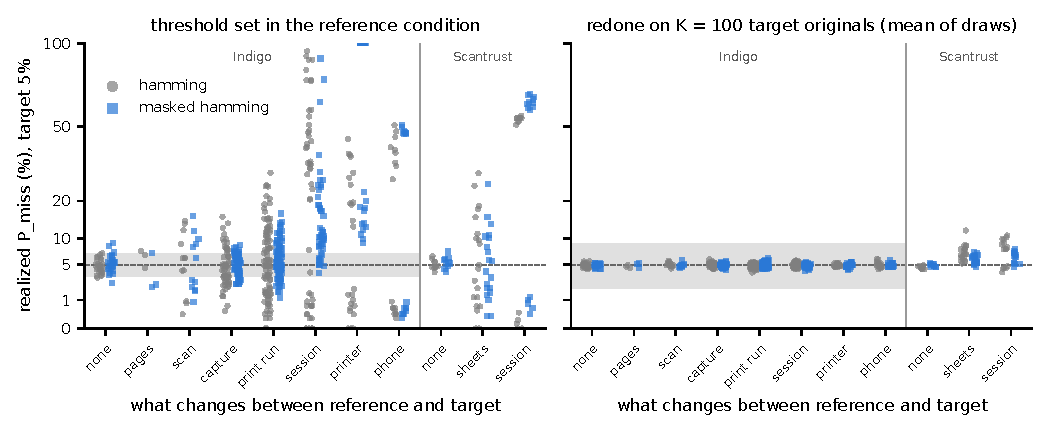
\includegraphics[width=\textwidth]{fig2.pdf}
  \caption{\todo{caption of Fig.~2.}}
  \label{fig:transfer}
\end{figure*}
\todo{results of Fig.~\ref{fig:transfer}.}

\subsection{Which test against which attacker}
\IfFileExists{figures/fig3.pdf}{%
\begin{figure}[t]
  \centering
  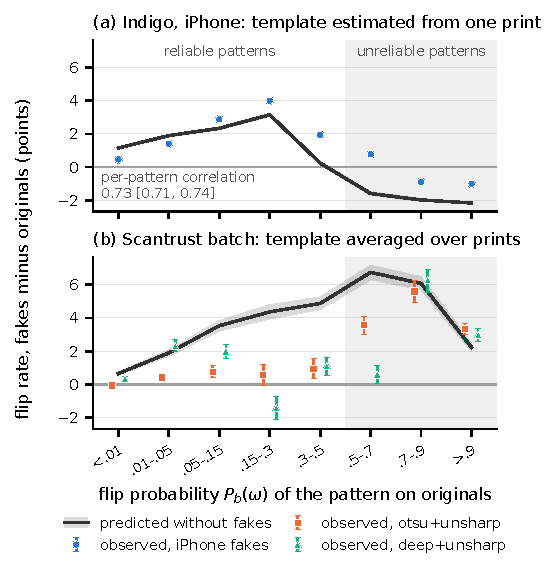
\includegraphics[width=\columnwidth]{fig3.pdf}
  \caption{\todo{caption of Fig.~3.}}
  \label{fig:twopass}
\end{figure}}{}

% Written by experiments/table1.py from the test-stage results:
%   c3a_9cf8e64f_test.json: git d9b576af14f3d2792c450a4cf02562832b7b6089
%   c3c_22649601_test.json: git d9b576af14f3d2792c450a4cf02562832b7b6089
%   p1_3f59ea51_test.json: git d9b576af14f3d2792c450a4cf02562832b7b6089
%   p2_9ab82b5b_test.json: git d9b576af14f3d2792c450a4cf02562832b7b6089
%   p3_1224833c_test.json: git d9b576af14f3d2792c450a4cf02562832b7b6089
\begin{table*}[t]
  \centering
  \definecolor{pfa}{HTML}{D6604D}
  \providecommand{\tcell}[4]{\begin{tabular}[t]{@{}c@{}}{\setlength{\fboxsep}{1.2pt}\colorbox{pfa!#1}{\makebox[4.6em]{\strut #2}}}\\[-2.5pt]{\fontsize{5.5}{6}\selectfont #3\enspace\textit{#4}}\end{tabular}}
  \caption{False-acceptance rate $\Pfa$ (\%) at a target $\Pmiss$ of 5\,\%: threshold set on originals only, test templates judged once}
  \label{tab:detection}
  \footnotesize
  \setlength{\tabcolsep}{3.5pt}
  \renewcommand{\arraystretch}{1.05}
  \begin{tabular}{@{}l cc cc cc@{}}
    \toprule
    & \multicolumn{2}{c}{Indigo, phone} & \multicolumn{2}{c}{Indigo, scanner: fakes on} & \multicolumn{2}{c}{Scantrust batch (averaging)} \\
    \cmidrule(lr){2-3} \cmidrule(lr){4-5} \cmidrule(lr){6-7}
    & iPhone & Samsung & same printer & other printer & otsu+unsharp & deep+unsharp \\
    \midrule
    \multicolumn{7}{@{}l}{\textit{Scores without fakes}} \\[1pt]
    Hamming distance & \tcell{32}{58.0}{[55.0, 60.8]}{5.4} & \tcell{53}{95.5}{[94.1, 96.6]}{6.7} & \tcell{55}{34.6--100.0}{range}{4.2--4.9} & \tcell{55}{47.6--99.8}{range}{4.2--4.9} & \tcell{34}{61.6}{[51.6, 71.2]}{5.9} & \tcell{30}{54.0}{[43.7, 64.3]}{5.9} \\
    Pearson correlation & \tcell{27}{49.8}{[46.9, 52.7]}{5.1} & \tcell{52}{93.9}{[92.4, 95.2]}{6.4} & \tcell{40}{4.6--72.2}{range}{4.2--4.4} & \tcell{32}{17.1--58.1}{range}{4.2--4.4} & \tcell{24}{44.1}{[33.3, 55.1]}{7.0} & \tcell{0}{\textbf{0.5}}{[0.0, 1.5]}{7.0} \\
    posterior log-likelihood & \tcell{1}{1.0}{[0.5, 1.7]}{5.0} & \tcell{48}{87.5}{[85.5, 89.4]}{6.6} & \tcell{0}{0.0--0.5}{range}{5.1--6.0} & \tcell{31}{0.0--56.8}{range}{5.1--6.0} & \tcell{55}{99.6}{[99.0, 100.0]}{6.5} & \tcell{52}{93.9}{[87.9, 98.7]}{6.5} \\
    masked Hamming ($\mu=0.01$, thesis) & \tcell{0}{0.3}{[0.1, 0.9]}{4.8} & \tcell{38}{69.4}{[66.6, 72.0]}{6.5} & \tcell{0}{\textbf{0.0}}{range}{5.1--5.3} & \tcell{0}{\textbf{0.0}}{range}{5.1--5.3} & \tcell{54}{97.8}{[96.0, 99.1]}{6.8} & \tcell{47}{85.4}{[78.9, 91.1]}{6.8} \\
    binned Mahalanobis & \tcell{19}{33.8}{[31.0, 36.6]}{4.5} & \tcell{46}{83.9}{[81.6, 85.9]}{4.7} & \tcell{4}{0.0--7.4}{range}{4.4--4.6} & \tcell{0}{\textbf{0.0}}{range}{4.4--4.6} & \tcell{25}{45.1}{[34.7, 55.7]}{5.6} & \tcell{10}{17.3}{[10.1, 25.4]}{5.6} \\
    \midrule
    \multicolumn{7}{@{}l}{\textit{Extensions without fakes}} \\[1pt]
    mask, $5\times5$ context$^\dagger$ & \tcell{0}{0.1}{[0.0, 0.5]}{4.6} & \tcell{31}{55.8}{[52.9, 58.7]}{6.7} & \tcell{0}{\textbf{0.0}}{range}{5.6} & \tcell{0}{\textbf{0.0}}{range}{5.6} & \tcell{51}{92.2}{[87.2, 96.2]}{7.9} & \tcell{36}{66.3}{[56.8, 75.5]}{7.9} \\
    mask, $3\times3$ context$^\dagger$ & \tcell{0}{0.1}{[0.0, 0.5]}{5.0} & \tcell{38}{69.7}{[67.0, 72.3]}{6.3} & \tcell{0}{\textbf{0.0}}{range}{4.6--5.8} & \tcell{0}{0.0--0.2}{range}{4.6--5.8} & \tcell{48}{87.8}{[81.7, 92.9]}{9.1} & \tcell{37}{68.2}{[58.6, 77.2]}{9.1} \\
    Hamming, same positions$^\dagger$ & \tcell{32}{57.6}{[54.7, 60.5]}{5.0} & \tcell{52}{95.4}{[94.0, 96.5]}{6.8} & \tcell{55}{33.9--100.0}{range}{4.4--4.9} & \tcell{55}{46.4--99.8}{range}{4.4--4.9} & \tcell{22}{40.0}{[29.9, 50.5]}{6.5} & \tcell{29}{53.0}{[42.6, 63.5]}{6.5} \\
    likelihood ratio, averaging attacker & -- & -- & -- & -- & \tcell{2}{\textbf{4.5}}{[1.9, 7.5]}{6.2} & \tcell{50}{91.3}{[84.9, 96.4]}{6.2} \\
    masked Hamming, one capture$^\ddagger$ & \tcell{0}{0.2}{[0.0, 0.6]}{4.8} & \tcell{34}{62.0}{[59.1, 64.8]}{6.7} & -- & -- & -- & -- \\
    masked Hamming, best of three captures & \tcell{0}{\textbf{0.0}}{[0.0, 0.3]}{5.3} & \tcell{0}{\textbf{0.3}}{[0.1, 0.9]}{6.2} & -- & -- & -- & -- \\
    \midrule
    \multicolumn{7}{@{}l}{\textit{Oracle: trained with fakes}} \\[1pt]
    logistic, same condition & \tcell{0}{0.4}{[0.1, 1.0]}{5.0} & \tcell{9}{17.1}{[15.0, 19.4]}{4.7} & \tcell{0}{0.0}{range}{4.2--5.1} & \tcell{0}{0.0}{range}{5.1--6.3} & \tcell{5}{8.8}{[4.0, 14.7]}{5.8} & \tcell{1}{1.1}{[0.4, 2.1]}{5.6} \\
    logistic, other condition$^\S$ & \tcell{9}{16.1}{[14.0, 18.4]}{4.4} & \tcell{31}{55.6}{[52.6, 58.5]}{6.6} & \tcell{8}{0.0--13.9}{range}{5.1--6.3} & \tcell{48}{0.0--87.2}{range}{4.2--5.1} & \tcell{42}{77.0}{[68.2, 84.3]}{6.6} & \tcell{36}{65.4}{[55.4, 74.7]}{6.6} \\
    \bottomrule
  \end{tabular}
  \par\vspace{3pt}
  \parbox{\textwidth}{\scriptsize Second line: 95\,\% CI (Clopper-Pearson on Indigo, bootstrap over templates on Scantrust), then the realized $\Pmiss$ (\%) in italics. Scanner columns: range over the two printers of the originals and the two template estimates. Shading grows with $\Pfa$; bold: lowest $\Pfa$ without fakes in the column. $^\dagger$Positions where the context masks can be learned; on Scantrust they leave out the frame, so these rows do not compare with the masked Hamming row. $^\ddagger$Codebook block of the three-capture experiment, not that of the rows above. $^\S$Other phone, fakes of the other printer, another Scantrust session; $C=10$ chosen by cross-validation, and over the grid $C\in\{10^{-3},\dots,10^{2}\}$: 66.4--98.9 (otsu+unsharp), 58.0--96.0 (deep+unsharp).}
\end{table*}

\todo{results of Table~\ref{tab:detection}.}

% ---------------------------------------------------------------------------- 0.5 page
\section{Discussion and limitations}
\todo{what this changes for provable guarantees; limitations (3 printers, 7 session pairs, 2 phones; Scantrust frame; fakes in one session per dataset); what did not work.}

% ------------------------------------------------- outside the page limit from here on
\section*{Ethical risks}
\todo{200 to 400 words: overconfident deployment; stakeholders; how we measured it; what we did about it; dual use.}

\bibliographystyle{IEEEtran}
\bibliography{references}

\appendix
\section*{Use of AI tools}
\todo{written by the team.}

\end{document}
